\chapter{Análise clássica para coloração em Grafos$(r,\ell)$}

\section{Exploração do problema de coloração mínima em Grafos$(r,\ell)$}
O problema de coloração aplicado a Grafos$(r,\ell)$ é de fácil solução para algumas especificações,
por exemplo um Grafo vazio, que é um Grafo(0,0) pode ser colorido com 0 cores, um Grafo disperso i.e um Grafo(1,0) é colorível com apenas uma cor, já que não existem arestas nesse grafo.

Já um Grafo completo, ou seja um Grafo(0,1), é colorível com K cores onde K é a quantidade de vértices nesse grafo completo, em um Grafo split que é um Grafo(1,1) essa regra se repete, já que cada vértice do conjunto independete pode ser colorível com alguma cor já presente na clique.

%primeira tabela de dicotomia
\begin{table}[!htb]
	\center
	\begin{tabular}{l|*{7}c}
		\toprule
		\backslashbox{$r$}{$l$} & 0 & 1 & 2 & 3 & 4 & \ldots & n\\
		\midrule
		0 & \P & \P & ? & ? & ? & \ldots & ?\\
		1 & \P & \P & ? & ? & ? & \ldots & ?\\
		2 & \P & ? & ? & ? & ? & \ldots & ?\\
		3 & ? & ? & ? & ? & ? & \ldots & ?\\
		4 & ? & ? & ? & ? & ? & \ldots & ?\\
		$\vdots$ & $\vdots$ & $\vdots$ & $\vdots$ & $\vdots$ & $\vdots$ & $\ddots$ & ?\\
		n & ? & ? & ? & ? & ? & \ldots & ?\\
		\bottomrule
	\end{tabular}%
	\caption{1ª Dicotomia parcial do problema de coloração em Grafos$(r,\ell)$}
	\label{tab:tabela_part1dictrl}%
\end{table}%

E por fim, Grafos bipartidos são coloridos com 2 cores uma cor para cada conjunto independente.

Sabemos então que coloração é de solução polinomial para grafos completos, dispersos, split e para grafos bipartidos. Assim sendo, temos como ponto de partida para a exploração futura da complexidade de Grafos de cardinalidade superiores a Tabela \ref{tab:tabela_part1dictrl}, a ser preenchida de acordo com os seguintes resultados.

%Teorema que coloração em (3,0) e (0,2) são polinomiais e (4,0) é NPc 
	\begin{teorema}
		Coloração de Grafo(0,2) é Polinomial.
	\end{teorema}
	\begin{proof}
		Um Grafo(0,2) é um grafo separável em 2 cliques, e que todo vértice faz parte de alguma das cliques, logo conhecer a clique máxima é simples e tendo a clique máxima sabemos que o numero mínimo de cores que pode ser usado para colorir o grafo é a cardinalidade da clique máxima.
	\end{proof}

	\begin{teorema}
		Coloração de Grafo(3,0) é Polinomial.
	\end{teorema}
	\begin{proof}
		Tendo um Grafo G da classe (3,0) como entrada para o problema de coloração sabemos então que o grafo pode ser colorido com 3 cores, resta saber se 3 é o o número mínimo de cores que pode ser usado, portanto devemos verificar se G é bipartido (colorível com duas cores) ou um grafo sem arestas (colorível com uma cor), como ambas verificações são polinomiais podemos afirmar que coloração de Grafo(3,0) é resolvível de forma polinomial.
	\end{proof}

	\begin{teorema}
		Coloração de Grafo(4,0) é NP-Completo.
	\end{teorema}
	\begin{proof}
		Sabemos que todo grafo planar é 4-colorível, e que alguns Grafos(4,0) são planares, portanto sabemos que para qualquer Grafo G $\in$ subconjunto de planares de Grafos(4,0), sua quantidade máxima de cores é 4, nos resta saber se 4 também é sua quantidade mínima, porém 3-coloração de planar é NP-Completo logo descobrir a coloração mínima de G é NP-Completo e consequentemente coloração de Grafos(4,0) é NP-Completo
	\end{proof}

É importante notar aqui que, todo $Grafo(r,\ell)$ é simultaneamente um $Grafo(r,\ell+1)$ já que podemos formar uma nova clique trivial utilizando qualquer vértice, e um $Grafo(r+1,\ell)$ já que podemos formar um novo conjunto independente trivial a partir de qualquer vértice, portanto se o problema de coloração é NP-Completo para um $Grafo(r,\ell)$ então ele é NP-Completo para qualquer $Grafo(r+1,\ell)$ ou $Grafo(r,\ell+1)$ .

Esses resultados nos levam à preencher a dicotomia da forma mostrada na Tabela \ref{tab:tabela_part2dictrl}
%Segunda tabela de dicotomia
\begin{table}[htb!]
	\center
	\begin{tabular}{l|*{7}c}
		\toprule
		\backslashbox{$r$}{$l$} & 0 & 1 & 2 & 3 & 4 & \ldots & n\\
		\midrule
		0 & \P & \P & \P & ? & ? & \ldots & ?\\
		1 & \P & \P & ? & ? & ? & \ldots & ?\\
		2 & \P & ? & ? & ? & ? & \ldots & ?\\
		3 & \P & ? & ? & ? & ? & \ldots & ?\\
		4 & \NPc & \NPc & \NPc & \NPc & \NPc & \ldots & \NPc\\
		$\vdots$ & $\vdots$ & $\vdots$ & $\vdots$ & $\vdots$ & $\vdots$ & $\ddots$ & \NPc\\
		n & \NPc & \NPc & \NPc & \NPc & \NPc & \ldots & \NPc\\
		\bottomrule
	\end{tabular}%
	\caption{2ª Dicotomia parcial do problema de coloração em Grafos$(r,\ell)$}
	\label{tab:tabela_part2dictrl}%
\end{table}%

Ainda nos falta mostrar a complexidade para alguns casos de fronteira, que necessitam de uma demonstração mais complexa.
%Demonstrar lista-coloração(r,l)Npc -> coloração(r,l+1)Npc e seus colorários (1,2) & (2,1)

Iremos demonstrar abaixo a complexidade para tais casos utilizando o seguinte teorema. 
\begin{teorema}
	Uma solução de lista coloração para um grafo$(r,\ell)$ $G$, implica em uma solução para o problema de coloração de um Grafo$(r,\ell+1)$ $H_G$
\end{teorema}
\begin{proof}
	Para a demonstração é preciso mostrar que
	\begin{itemize}
		\item Se um grafo G$(r,\ell)$ possui uma lista coloração própria então $H_G$ é k-colorível para k do tamanho da paleta $P$ (1)
		\item Se $H_G$ é k-colorível então G possui uma lista coloração própria (2)
	\end{itemize}
	(1):\newline
	
	Usaremos a seguinte construção:\newline
	Considere G um grafo$(r,\ell)$ e que para cada vértice $v \in V(G)$ exista uma lista de cores $S_v$ referente a esse vértice, cada lista contém pelo menos uma cor do conjunto $C = \{c_1,c_2,c_3,...,c_k \}$, sendo G uma instância sim para o problema de lista coloração, criemos uma clique K onde cada vértice $k \in V(K)$ representa uma cor presente em $C$. Seja $H_G = G \cup K$ para todo vértice $v \in G$ e todo vértice $u_i \in K$ adicione uma aresta $(u_i,v)$ à $H_G$ se e somente se v não possui a cor $c_i$ em sua lista coloração em G
	
	Podemos então generalizar da seguinte forma, dado um grafo$(r,\ell)$ $G$ onde cada vértice de $G$ possui uma lista de possíveis cores então o grafo $H_G$ obtido pela construção anterior possui uma k-coloração.
	
	Note que a clique K possui exatamente k vértices, consequentemente para colorirmos K precisaremos de k cores, sem perda de generalidade assumimos que $u_1$ será colorido com $c_1$, $u_2$ com $c_2$ e assim por diante.
	
	Por construção uma aresta de $u_i$ só existe para $v_a$ em $H_G$ se e somente se, $v_a$ não possui $c_i$ em sua lista de cores, portanto a coloração atribuída à K não conflita com a com a lista coloração de G, e portanto para todo vértice perntecente a G podemos lhe atribuir a mesma cor que lhe foi atribuída no problema de lista coloração, obtendo uma coloração própria mínima para $H_G$
	
	(2):\newline
	Suponha que o grafo $H_G$ possua uma K-coloração própria, onde k é o número de cores nas listas de G
	
	Seja K a maior clique presente em $H_G$, por construção $H_G$ é colorível com k cores onde k é a cardinalidade de K, observe que a remoção de K não afeta a coloração de $H_G - K$
	
	Como $H_G$ é k-colorível e a clique K possui k vértices todas as cores de tal k-coloração estão presentes em K. Sem perda de generalidade podemos assumir que as cores $c_1,c_2,...,c_k$ estão atribuídas aos vértices $u_1,u_2,...,u_k$ pertencentes à K
	
	Por construção de $H_G$ todo par $(v,u_i)$ onde $v \in H_G - K$ e $u_i \in K$ é não adjacente se e somente se o vértice $v$ não possui $c_i$ em sua lista coloração no grafo $G$
	
	Logo a k-coloração atribuídas aos vértices em $H_G - K$ formam uma coloração para G onde todo vértice em $V(G)$ possui uma cor de sua lista. Portanto G é uma instância sim de lista coloração
\end{proof}
\begin{corolario}
	Se lista coloração é NP-Completo para Grafos split então coloração é NP-Completo para Grafos$(1,2)$.
	\begin{proof}
		A NP-Completude de lista coloração em grafos split é demonstrado por Jensen et al.\cite{jansen1997}
	\end{proof}
\end{corolario}
\begin{corolario}
	Se Lista coloração é NP-Completo em Grafos(2,0) então Coloração é NP-Completo em Grafos$(2,1)$.
	\begin{proof}
		A NP-Completude de lista coloração em grafos bipartido é demonstrado por Fellows et al. em "List Coloring and Precoloring Extension are W[1]-hard parameterized by treewidth"
	\end{proof}
\end{corolario}    
\begin{corolario}
	Se lista coloração é NP-Completo para Grafos(0,2) então Coloração é NP-Completo em Grafos(0,3).
	\begin{proof}
		Para essa demonstração nos basearemos em um resultado obtido por Jensen em "Complexity results for the optimum cost chromatic partition problem". a demonstração se baseia em realizar uma redução do problema 3-SAT restrito para lista coloração de co-bipartido i.e. Grafo(0,2).
		Suponha o problema 3-SAT com as seguintes restrições:
		\begin{itemize}
			\item cada cláusula $c_i$ contém dois ou três literais.
			\item cada literal ou sua negação aparece no máximo em 3 cláusulas
		\end{itemize}
		Construiremos agora uma instância de lista coloração da seguinte forma:\newline
		Para cada varíavel $j$ crie seis vértices:
		$a_j^{(1)}$, $a_j^{(2)}$, $a_j^{(3)}$;
		$b_j^{(1)}$, $b_j^{(2)}$, $3_j^{(3)}$. Atribuindo a cada uma lista de cores da seguinte forma:\newline
		$a_j^{(k)}$ <= \{$x_j^{(k)}$, $\overline{x_j}^{(k)}$ \}; $b_j^{(k)}$ <= \{$\overline{x_j}^{(k)}$,$x_j^{((k \Mod{3}) + 1 )}$ \}\newline
		Definimos como A o conjunto de todos os $a_j^{(k)}$ e B o conjunto de todos os $b_j^{(k)}$ e construímos uma clique com os vértices de A e B. Observe que só existem duas maneiras de se colorir este grafo:
		\begin{itemize}
			\item (1)  $f(a_j^{(k)}) = x_j^{(k)} => b_j^{(k)} = \overline{x_j}^{(k)}$
			\item (2)  $f(a_j^{(k)}) = \overline{x_j}^{(k)} => b_j^{(k)} = x_j^{((k \Mod{3}) + 1 )}$
		\end{itemize}
		Agora, para cada cláusula definimos um vértice $c_i$ e sua lista de cores da seguinte forma: para cada literal $j$ ou sua negação $\overline{j}$ presente na cláusula adicionamos à lista de $c_i$ o $x_j^{(k)}$ onde k é o indice de ocorrência do literal ou de sua negação.
		
		Por exemplo, suponha o seguinte 3-SAT:
		
		$(p \lor q \lor r) \land (\neg{p} \lor q \lor r) \land (\neg{p} \lor \neg{r} \lor s)$
		
		suas cláusulas seriam traduzidas para
		\begin{itemize}
			\item $c_1$ com lista: \{$p^1$, $q^1$, $r^1$ \}
			\item $c_2$ com lista: \{$\overline{p}^2$, $q^2$, $r^2$ \}
			\item $c_3$ com lista: \{$\overline{p}^3$, $\overline{r}^3$, $s^1$ \}
		\end{itemize}
		Seja C o conjunto contendo todos os $c_i$ criamos uma clique com $C \cup A$.
		Nosso grafo tem portanto a seguinte configuração(considere $x'$ como $\overline{x}$):
		\begin{figure}[!ht]
			\centering
			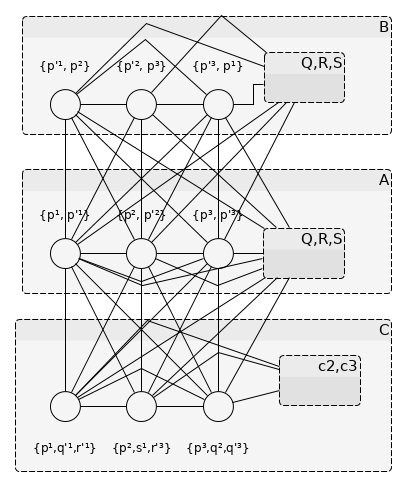
\includegraphics[width=0.6\textwidth]{3-SAT.png}
			\caption{Grafo G: Transformaçao de 3-SAT em co-bipartido }
		\end{figure}
		
		Suponha a cláusula p, se p é falso então $a_p^{(1)},a_p^{(2)},a_p^{(3)}$ será colorido com $p^1,p^2,p^3$ respectivamente
		
		Dessa forma mostramos que o o grafo construído só tem solução para lista coloração se existe pelo menos um literal verdadeiro em todas as cláusulas
	\end{proof}
\end{corolario}
Portanto podemos agora completar nossa tabela com:
\newpage
\begin{table}[!htb]
	\center
	\begin{tabular}{l|*{7}c}
		\toprule
		\backslashbox{$r$}{$l$} & 0 & 1 & 2 & 3 & 4 & \ldots & n\\
		\midrule
		0 & \P & \P & \P & \NPc & \NPc & \ldots & \NPc\\
		1 & \P & \P & \NPc & \NPc & \NPc & \ldots & \NPc\\
		2 & \P & \NPc & \NPc & \NPc & \NPc & \ldots & \NPc\\
		3 & \P & \NPc & \NPc & \NPc & \NPc & \ldots & \NPc\\
		4 & \NPc & \NPc & \NPc & \NPc & \NPc & \ldots & \NPc\\
		$\vdots$ & $\vdots$ & $\vdots$ & $\vdots$ & $\vdots$ & $\vdots$ & $\ddots$ & \NPc\\
		n & \NPc & \NPc & \NPc & \NPc & \NPc & \ldots & \NPc\\
		\bottomrule
	\end{tabular}%
	\caption{Dicotomia do problema de coloração em Grafos$(r,\ell)$}
	\label{tab:tabela_dictrl}%
\end{table}%
